\chapter{电磁能量与坡印廷矢量}\label{ch:b2:poynting-vector}

电池通过两根铜线点亮一只灯泡。能量沿
何处传递？答案并不在铜线之内：那里的电子
以约每秒一毫米的速度漂移，几乎不携带能量。
能量沿\emph{导线周围的空间}流动，
即在电磁场中，并经灯丝的
侧面进入灯丝。太阳也以这种方式，向晴朗屋顶的每平方米
输送一千瓦，穿越一亿五千万千米的
真空。本章由麦克斯韦方程组推出电磁能量的
收支表——场中储存多少能量，以及
指明能量去向的矢量——坡印廷矢量——并将其用于
一根导线、一个电容器、一只线圈和一束光。

\section{场的能量平衡}

\begin{theorem}[坡印廷定理]\label{thm:b2:poynting-vector:poynting}
\index{坡印廷矢量}\index{坡印廷定理}\index{电磁能量密度}
定义\emph{电磁能量密度}和\emph{坡印廷
矢量}
\[
u = \frac{\varepsilon_0E^2}2 + \frac{B^2}{2\mu_0} \quad (\unit{J/m^3}) , \qquad
\vect\Pi = \frac{\vect E\wedge\vect B}{\mu_0} \quad (\unit{W/m^2}) .
\]
麦克斯韦方程组在每一点蕴含
\[
\frac{\partial u}{\partial t} + \operatorname{div}\vect\Pi = -\vect j\cdot\vect E ,
\]
对任一固定体积 $V$，其边界为 $\Sigma$，
\[
\frac{\dd}{\dd t}\iiint_Vu\,\dd\tau = -\iint_\Sigma\vect\Pi\cdot\vect n\,\dd S - \iiint_V\vect j\cdot\vect E\,\dd\tau :
\]
$V$ 内场的能量减少，减少量一为经边界
流出的部分（$\vect\Pi$ 的通量），二为场传给电荷的
部分（$\vect j\cdot\vect E$，即导体中的焦耳功率）。$\vect\Pi$ 为
能流密度，即与之垂直的单位面积上
穿过的功率。
\end{theorem}

\begin{proof}
由麦克斯韦–安培方程，$\vect j = \operatorname{\vect{curl}}\vect B/\mu_0 - \varepsilon_0\partial_t
\vect E$，于是 $\vect j\cdot\vect E = \vect E\cdot\operatorname{\vect{curl}}\vect B/\mu_0 -
\partial_t(\varepsilon_0E^2/2)$。恒等式 $\operatorname{div}(\vect E\wedge\vect B) = \vect B
\cdot\operatorname{\vect{curl}}\vect E - \vect E\cdot\operatorname{\vect{curl}}\vect B$（可逐分量
验证），由麦克斯韦–法拉第方程可得 $\vect E\cdot\operatorname{\vect{curl}}
\vect B = -\operatorname{div}(\vect E\wedge\vect B) - \vect B\cdot\partial_t\vect B = -\mu_0
\operatorname{div}\vect\Pi - \partial_t(B^2/2)$。合并得 $\vect j\cdot\vect E = -\operatorname{div}
\vect\Pi - \partial_tu$。对 $V$ 积分，并应用散度定理。
\end{proof}

\begin{remark}[哪些是确定的，哪些不是]\label{rem:b2:poynting-vector:interpretation}
定理只确定 $\vect\Pi$ 穿过闭合曲面的通量
以及总量 $u$；若在 $\vect\Pi$ 上加一个无散场，
则不改变任何可观测量。上面的取法最简单，
与光携带的动量相符（见下文），而且它
已被普遍采用。两个密度 $\varepsilon_0E^2/2$ 与 $B^2/2\mu_0$ 恰是
本科一年级分册中电容器与电感器的能量，
现在赋予空间每一点：电场强度为 \qty{1}{MV/m}（空气的
击穿极限）的场储存 \qty{4.4}{J/m^3}；磁场为 \qty{1}{T}
时则储存 \qty{0.4}{MJ/m^3}——高出十万倍，
这正是磁铁而非电容器能够储存兆焦耳能量的原因。
\end{remark}

\section{能量的流向：三个电路}

\begin{example}[有电阻的导线]\label{ex:b2:poynting-vector:wire}
半径为 $a$ 的圆柱形导线通有恒定电流 $I$，在
沿轴向的电场 $E = j/\gamma$ 作用下；导线外紧邻处，$B = \mu_0I/2\pi a$
（方位向）。表面处，$\vect\Pi = \vect E\wedge\vect B/\mu_0$ 指向
\emph{沿径向向内}，大小为 $EI/2\pi a$；其穿过
长为 $L$ 的侧面的通量为 $EI/2\pi a\times2\pi aL = (EL)I = UI =
RI^2$：焦耳热经导线侧面进入，由
周围的场输送，而非由电子沿导线输运。
在内部，$\Pi(r) = (E/\mu_0)(\mu_0Ir/2\pi a^2) = EIr/2\pi a^2$：向内的能流
随靠近轴线而减小，即能量逐层沉积。
\end{example}

\begin{example}[电容器与螺线管]\label{ex:b2:poynting-vector:capsol}
一个圆形极板的电容器正在充电：$\vect E$ 沿轴向，$\vect B =
\mu_0\varepsilon_0(r/2)\dot E\,\vect e_\theta$（见\cref{ch:b2:maxwell-equations}），于是
$\vect\Pi = -\varepsilon_0(r/2)E\dot E\,\vect e_r$，方向向内；穿过
半径为 $R$、高为 $d$ 的圆柱面，其通量为 $\varepsilon_0\pi R^2d\,E\dot E = \dd(\tfrac12
\varepsilon_0E^2\,\pi R^2d)/\dd t$：电能从边缘进入。一个
螺线管，其电流增大：$\vect B$ 沿轴向，感生的 $\vect E = -(r/2)
\dot B\,\vect e_\theta$，$\vect\Pi = -(rB\dot B/2\mu_0)\vect e_r$，仍向内，
通量为 $\dd(B^2/2\mu_0\times\text{体积})/\dd t$。各种情形下，能量
经器件外部的场到达器件；导线只是
引导场。
\end{example}

\begin{omfigure}
\begin{tikzpicture}[font=\small, x=1cm, y=1cm, >=Stealth]
  \begin{scope}
    \draw[thick, fill=omExo!20] (-2.4,-0.5) rectangle (2.4,0.5);
    \draw[omDef, thick, ->] (-1.6,0) -- (-0.6,0) node[above, font=\footnotesize] {$\vect E$};
    \draw[omDef, thick, ->] (0.6,0) -- (1.6,0);
    \node[omProp, font=\footnotesize] at (0,0.8) {$\odot\ \vect B$}; \node[omProp, font=\footnotesize] at (0,-0.8) {$\otimes\ \vect B$};
    \foreach \x in {-1.8,-0.9,0,0.9,1.8} {\draw[omThm, thick, ->] (\x,1.4) -- (\x,0.6); \draw[omThm, thick, ->] (\x,-1.4) -- (\x,-0.6);}
    \node[omThm, font=\footnotesize] at (2.5,1.1) {$\vect\Pi$};
    \node[font=\footnotesize] at (0,-1.85) {导线：$\vect\Pi$ 向内，通量 $= RI^2$};
  \end{scope}
  \begin{scope}[xshift=7.2cm]
    \draw[thick, fill=omExo!40] (-0.9,-1.3) rectangle (-0.75,1.3); \draw[thick, fill=omExo!40] (0.75,-1.3) rectangle (0.9,1.3);
    \foreach \y in {-0.9,-0.45,0,0.45,0.9} \draw[omDef, ->] (-0.7,\y) -- (0.7,\y);
    \node[omDef, font=\footnotesize] at (0,1.55) {$\vect E$ 增大};
    \foreach \y in {-1.0,-0.5,0,0.5,1.0} {\draw[omThm, thick, ->] (1.9,\y) -- (1.05,\y); \draw[omThm, thick, ->] (-1.9,\y) -- (-1.05,\y);}
    \node[omThm, font=\footnotesize] at (2.2,1.3) {$\vect\Pi$};
    \node[font=\footnotesize] at (0,-1.85) {电容器：能量从边缘进入};
  \end{scope}
\end{tikzpicture}

{\small 左：载流导线——由轴向 $\vect E$ 与周向 $\vect B$ 构成的坡印廷矢量，
处处指向导线表面；
焦耳热经侧面进入导线。右：
正在充电的电容器——能量沿径向穿过间隙流入，
而不经过极板。}
\end{omfigure}

\begin{remark}[静止正交场中的能量]\label{rem:b2:poynting-vector:static}
将一带电电容器置于永磁体的场中，
则两极板之间处处有 $\vect\Pi = \vect E\wedge\vect B/\mu_0 \ne \vect 0$，
虽然一切都不变化，也不发热。这并无矛盾：
此处 $\vect\Pi$ 的散度为零，其场线自成闭合，
穿过任一闭合曲面的通量为零——定理并未涉及
一种不输送任何能量的环流。只有穿过闭合曲面的通量
才有物理意义。
\end{remark}

\begin{omfigure}
\begin{tikzpicture}[font=\small, x=1cm, y=1cm, >=Stealth]
  \begin{scope}
    \draw[thick, fill=omExo!30] (0,0) circle (1.6); \draw[thick, fill=omDef!10] (0,0) circle (1.35); \draw[thick, fill=omExo!60] (0,0) circle (0.35);
    \foreach \a in {0,45,...,315} \draw[omDef, ->] ({0.4*cos(\a)},{0.4*sin(\a)}) -- ({1.1*cos(\a)},{1.1*sin(\a)});
    \draw[omProp, thick, ->] (0.85,0) arc[start angle=0, end angle=300, radius=0.85];
    \node[omDef, font=\footnotesize] at (1.0,1.35) {$\vect E$}; \node[omProp, font=\footnotesize] at (-0.55,-1.05) {$\vect B$};
    \node[font=\footnotesize] at (0,0) {$\odot$};
    \node[font=\footnotesize] at (0,-2.1) {芯线中电流指向读者：$\vect\Pi$ 亦指向读者};
  \end{scope}
  \begin{scope}[xshift=7.8cm]
    \draw[thick] (-2.6,0.3) -- (2.6,0.3) (-2.6,-0.3) -- (2.6,-0.3);
    \draw[thick] (-2.6,1.2) -- (2.6,1.2) (-2.6,-1.2) -- (2.6,-1.2);
    \fill[omDef!10] (-2.6,0.3) rectangle (2.6,1.2); \fill[omDef!10] (-2.6,-1.2) rectangle (2.6,-0.3);
    \fill[omExo!40] (-2.6,-0.3) rectangle (2.6,0.3);
    \foreach \y in {0.55,0.75,0.95} \draw[omThm, thick, ->] (-1.8,\y) -- (-0.4,\y);
    \foreach \y in {-0.55,-0.75,-0.95} \draw[omThm, thick, ->] (0.4,\y) -- (1.8,\y);
    \node[omThm, font=\footnotesize] at (-1.1,1.45) {$\vect\Pi$ 沿电缆方向，位于电介质中};
    \node[font=\footnotesize] at (0,0) {芯线};
    \node[font=\footnotesize] at (0,-2.1) {$\displaystyle\iint\vect\Pi\cdot\dd\vect S = UI$};
  \end{scope}
\end{tikzpicture}

{\small 输送功率的同轴电缆：径向的 $\vect E$ 与周向的
$\vect B$ 在电介质中形成轴向的坡印廷矢量，其穿过
两导体之间环形区域的通量恰为 $UI$——功率
在绝缘体中传输，金属只起导引作用。}
\end{omfigure}

\section{光：光强与辐射压强}

\begin{proposition}[平面波的能量]\label{prop:b2:poynting-vector:wave}
\index{光强（电磁）}\index{辐射压强}\index{辐照度}
对真空中的平面波——即\cref{ch:b2:plane-waves-polarization}中的解，
其中 $\vect B = \vect k\wedge\vect E/\omega$，$B = E/c$ 且 $\vect E \perp \vect B$——
电场与磁场的能量密度相等，且
\[
u = \varepsilon_0E^2 , \qquad \vect\Pi = \varepsilon_0cE^2\,\vect u = cu\,\vect u ,
\]
$\vect u$ 为传播方向，能量以 $c$ 的速率传播。
对振幅为 $E_0$ 的正弦波，\emph{光强}
（辐照度）即平均通量，
\[
I = \langle\Pi\rangle = \frac{\varepsilon_0cE_0^2}2 = \frac{E_0^2}{2\mu_0c} ,
\]
且波携带动量密度 $\vect\Pi/c^2$（在本阶段不加证明地承认），因此
它在垂直入射于某表面时，对该表面施加的
\emph{辐射压强} $P = I/c$（若被吸收）与 $2I/c$（若被反射）。
\end{proposition}

\begin{proof}
$B^2/2\mu_0 = E^2/2\mu_0c^2 = \varepsilon_0E^2/2$; $\vect E\wedge\vect B/\mu_0 = E^2/\mu_0c =
\varepsilon_0cE^2$ 沿 $\vect k$；$\langle\cos^2\rangle = \tfrac12$。动量
密度 $\vect\Pi/c^2$ 可由吸收表面中电荷所受的洛伦兹力导出
（或由相对论得 $p = E/c$，对光而言）：
$\Pi S\,\dd t/c^2\times c$ 为单位时间内到达表面 $S$ 的动量，
即作用力 $\Pi S/c$。
\end{proof}

\begin{example}[日光、激光与微波]\label{ex:b2:poynting-vector:orders}
大气层顶端的日光，$I = \qty{1.36}{kW/m^2}$：$E_0 =
\sqrt{2I/\varepsilon_0c} = \qty{1.0}{kV/m}$，$B_0 = E_0/c = \qty{3.4}{\micro T}$，能量
密度 \qty{4.5}{\micro J/m^3}，压强 \qty{4.5}{\micro Pa}——\qty{0.7}{kg}
的力作用于每平方千米，却足以操纵太阳帆，并
把彗星的尘埃吹成彗尾。一支 \qty{1}{mW} 的激光笔照在
\qty{1}{mm^2} 的光斑上：\qty{1}{kW/m^2}，与太阳相当；聚焦到 \qty{1}{\micro m^2} 时：
\qty{1}{GW/m^2}，$E_0 = \qty{0.9}{MV/m}$，接近空气的击穿强度。一台
\qty{1}{kW} 的微波炉内，驻波充满 $\qty{30}{L}$ 的体积：能量
密度 $\sim 10^{-7}$ J/m$^3$，$E_0$ 约为每米几千伏。
\end{example}

\begin{omfigure}
\begin{tikzpicture}[font=\small, x=1cm, y=1cm, >=Stealth]
  \draw[->, thick] (0,0) -- (6.2,0) node[right, font=\footnotesize] {$\vect u$（传播方向）};
  \foreach \x in {0.4,1.0,...,5.2} {
    \pgfmathsetmacro{\e}{1.2*sin(deg(1.4*\x))}
    \draw[omDef, ->] (\x,0) -- (\x,\e);
    \draw[omProp, ->] (\x,0) -- ({\x+0.45*\e},{-0.3*\e});
  }
  \node[omDef, font=\footnotesize] at (1.1,1.5) {$\vect E$};
  \node[omProp, font=\footnotesize] at (2.0,-0.75) {$\vect B$};
  \draw[omThm, very thick, ->] (2.5,-1.6) -- (4.5,-1.6) node[right, font=\footnotesize] {$\vect\Pi = \vect E\wedge\vect B/\mu_0$};
\end{tikzpicture}

{\small 平面电磁波：$\vect E$、$\vect B$ 与
传播方向构成右手系；坡印廷
矢量沿传播方向，并以两倍频率振荡，
其平均值即为光强。}
\end{omfigure}

\begin{method}[能量核算]\label{met:b2:poynting-vector:method}
(1) 求 $\vect E$ 与 $\vect B$（静态、准静态或波动情形）。(2)
写出 $\vect\Pi = \vect E\wedge\vect B/\mu_0$ 与 $u$。(3) 选取包围装置的闭合
曲面，计算 $\vect\Pi$ 的通量：它
应等于焦耳热功率与内部储能的变化率之和
——这是对场的一项检验。(4) 对于波，$\Pi$ 的平均值即为光强；
除以 $c$ 得压强，除以光子能量
$hf$ 得光子通量。
\end{method}

\section{练习}

\begin{exercise}[$\star$]\label{exo:b2:poynting-vector:1}
地面处的日光，$I = \qty{1.0}{kW/m^2}$：振幅 $E_0$ 与 $B_0$，
能量密度，黑色屋顶与镜子上的辐射压强；
面积为 \qty{100}{m^2} 的屋顶所受的力；每平方米的光子通量，
取平均光子能量为 \qty{2}{eV}。
\end{exercise}

\begin{exercise}[$\star$]\label{exo:b2:poynting-vector:2}
功率为 \qty{5}{mW} 的激光笔，光束直径 \qty{1.5}{mm}：光强、$E_0$、
$B_0$；将同一光束聚焦到 \qty{5}{\micro m} 的光斑上；一台 \qty{1}{PW}
（\qty{1e15}{W}）的脉冲激光器聚焦到 \qty{10}{\micro m^2} 的面积上：$E_0$，并与
氢原子中束缚电子的场（\qty{5e11}{V/m}）相比较。
\end{exercise}

\begin{exercise}[$\star$]\label{exo:b2:poynting-vector:3}
能量密度：电场为 \qty{3}{MV/m}（空气击穿）；
电场为 \qty{100}{MV/m}（薄绝缘体）；磁场为 \qty{0.1}{T}，
\qty{1.5}{T}（MRI），\qty{45}{T}（创纪录的磁体）。求体积为 \qty{1}{m^3} 的 MRI
孔道内的能量，以及以汽油升数计的等价量（\qty{35}{MJ/L}）。
\end{exercise}

\begin{exercise}[$\star$]\label{exo:b2:poynting-vector:4}
一张 \qty{100}{m} $\times$ \qty{100}{m} 的太阳帆，完全反射，位于
地球距离处（$I = \qty{1.36}{kW/m^2}$）：所受的力；
质量为 \qty{200}{kg} 的飞行器的加速度；一个月内获得的速率；
并与该处太阳对飞行器的引力（\qty{5.9e-3}{N/kg}）相比较。
\end{exercise}

\begin{exercise}[$\star\star$]\label{exo:b2:poynting-vector:5}
一根半径为 $a = \qty{1}{mm}$ 的铜线通有 \qty{10}{A} 的电流（$\gamma =
\qty{6e7}{S/m}$）。(a) 内部的 $E$，表面的 $B$，表面的 $\vect\Pi$（方向与大小）。
(b) 求 $\vect\Pi$ 流入 \qty{1}{m}
导线的通量，并与 $RI^2$ 相比较。(c) 导线内部的 $\Pi(r)$，以及
在 $r$ 与 $r + \dd r$ 之间沉积的功率；验证其等于 $j^2/\gamma\cdot2\pi r\,\dd r$。
(d) 能量从何处来——描述
电池与导线之间的场。
\end{exercise}

\begin{exercise}[$\star\star$]\label{exo:b2:poynting-vector:6}
圆形极板电容器（$R$，$d$）由电流 $I$ 充电。(a) 求 $\vect E$、$\vect B$，
以及两极板间的 $\vect\Pi$。(b) 求 $\vect\Pi$ 穿过侧面圆柱面的通量；
并证明其等于 $\dd W_e/\dd t$。(c) 取 $R = \qty{5}{cm}$，$d =
\qty{1}{mm}$，$I = \qty{1}{A}$，某时刻 $E = \qty{1}{MV/m}$：$\Pi$ 在
边缘处的大小与流入的功率。(d) 磁能能否忽略？
\end{exercise}

\begin{exercise}[$\star\star$]\label{exo:b2:poynting-vector:7}
一根长螺线管（$n$，半径 $R$），其电流 $I(t)$ 增大。(a)
求内部的感应 $\vect E$、$\vect\Pi$ 及其方向。(b) 求穿过
侧面单位长度的通量，以及 $\dd(B^2/2\mu_0\cdot\pi R^2)/\dd t$。(c)
恰在螺线管外侧（$\vect B = \vect 0$ 处），$\vect\Pi$ 是多少？
那么能量如何进入？（想一想电流在何处流动：
绕组是一薄层；取紧贴其内侧的表面。）
\end{exercise}

\begin{exercise}[$\star\star$]\label{exo:b2:poynting-vector:8}
\emph{功率沿何处传输。}同轴电缆（半径 $a$，
$b$）的芯线中通有恒定电流 $I$，经编织层流回，
两导体间电压为 $U$（理想导体）。(a) 求 $\vect E$ 与 $\vect B$
在电介质中（$a < r < b$）的表达式，由高斯定律与安培定律求得。(b) 求 $\vect\Pi$：
(c) 对 $\vect\Pi$ 在环形区域 $a < r
< b$ 积分，证明结果为 $UI$——全部功率
都在绝缘体中传输。(d) 若中芯略有电阻，
$\vect\Pi$ 向哪个方向偏斜，流入中芯的通量等于什么？
\end{exercise}

\begin{exercise}[$\star\star$]\label{exo:b2:poynting-vector:9}
\emph{彗星尘埃。}半径为 $a$、密度为
$\rho = \qty{2000}{kg/m^3}$ 的球形尘粒，位于距太阳 $D$ 处，吸收
日光（$I = \qty{1.36}{kW/m^2}$，在 $D_0 = \qty{1.5e11}{m}$ 处，太阳质量
为 \qty{2.0e30}{kg}）。(a) 求辐射力与引力，
并证明二者之比与 $D$ 无关。(b) 求临界半径，半径小于此值时
尘粒将被吹走。(c) 为何彗尾背向太阳，又为何
会弯曲？
\end{exercise}

\begin{exercise}[$\star\star\star$]\label{exo:b2:poynting-vector:10}
\emph{放电中的电容器。}\cref{exo:b2:poynting-vector:6}中的电容器
经\cref{exo:b2:poynting-vector:5}中的导线放电
（$R = \qty{5.3}{m\ohm}$ 每米，长度
$L$）。(a) 此刻电容器边缘处 $\vect\Pi$ 的方向。(b) 离开电容器的功率与
流入导线的功率；它们之差（若有）
去向如何？(c) 写出能量平衡 $\dd W_e/\dd t = -RI^2$
并与 $Q = CU$、$I = -\dd Q/\dd t$ 相核对。(d) 为何
电路的磁能在开始与结束时均不出现在
平衡式中？
\end{exercise}

\begin{exercise}[$\star\star\star$]\label{exo:b2:poynting-vector:11}
\emph{带电磁铁。}带电电容器两极板之间
（$\vect E = E\vect e_z$）放有均匀磁场 $\vect B = B\vect e_x$（一块磁铁）。
(a) 求 $\vect\Pi$ 及其散度。(b) 取区域内一个盒子的闭合曲面，
求 $\vect\Pi$ 的通量。(c) $\vect\Pi$ 的线去往何处，
又由什么使其闭合？(d) 有人提议，在间隙中放一个小吸收体以测量能流，
它会发热吗？为什么不会？
\end{exercise}

\begin{exercise}[$\star\star\star$]\label{exo:b2:poynting-vector:12}
\emph{驻波。}两列振幅相等、传播方向相反的平面波
叠加成 $\vect E = 2E_0\cos kx\cos\omega t\,\vect e_y$，$\vect B = -2(E_0/c)
\sin kx\sin\omega t\,\vect e_z$（对照麦克斯韦–法拉第方程检验）。(a)
求 $\vect\Pi(x, t)$ 及其时间平均。(b) 能量密度；何处为电能，何处为磁能，
能量如何来回转移？(c) 一面位于 $x = 0$ 处的理想导体镜
面反射入射波，其单位
面积所受的力可由动量论证得到，也可由作用于
其表面电流的拉普拉斯力得到（利用 $\vect B$ 的边界关系）。(d) 证明
二者的平均值均为 $2I/c$。
\end{exercise}

\begin{omfigure}
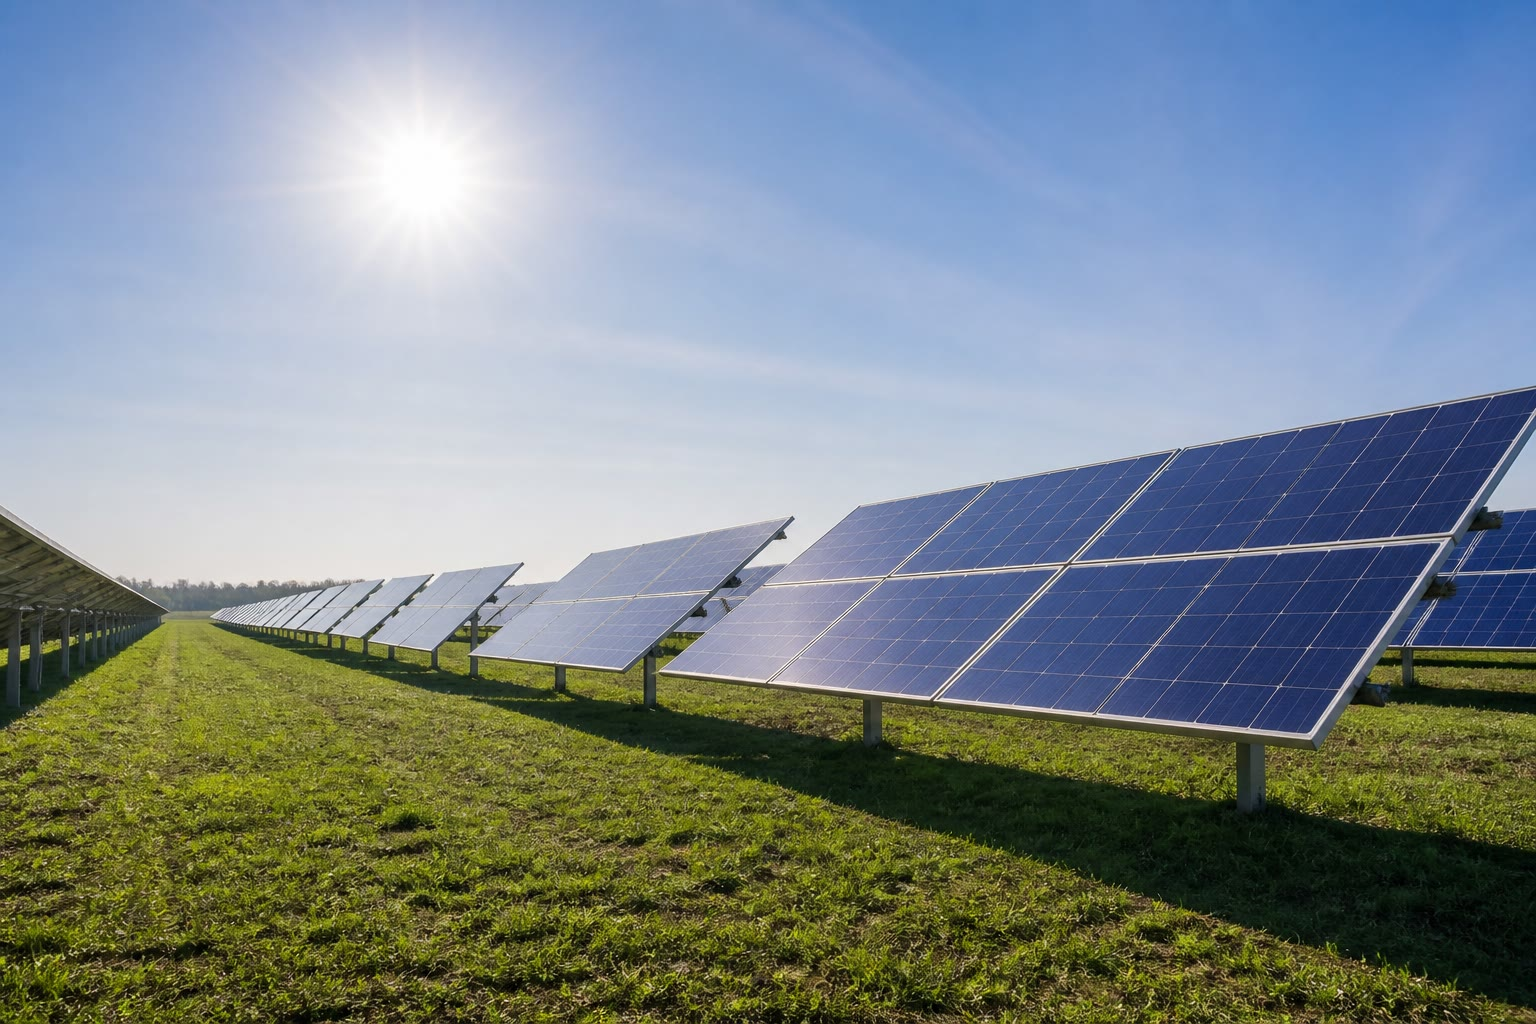
\includegraphics[width=0.58\linewidth]{images/book4/ai/b4-12-solar-farm-sun.jpg}

{\small 一座太阳能电站：每平方米有一千瓦的坡印廷通量自太阳穿越空旷空间抵达，其中五分之一经电缆输出。}
\end{omfigure}

\section{问题：线路、面板与烤箱中的能量}

\begin{problem}[{周末问题——追踪电磁能量
从输电线路进入住宅、从太阳进入太阳能板，
以及从磁控管进入一杯水中}]
\label{pb:b2:poynting-vector:1}

\medskip
\noindent\textbf{第一部分——线路。}
一根同轴电力电缆（芯线半径 $a = \qty{1.0}{cm}$，屏蔽层半径 $b =
\qty{3.0}{cm}$，电介质 $\varepsilon_r = 2.3$）载有直流电流 $I =
\qty{500}{A}$，电压为 $U = \qty{20}{kV}$；芯线的电导率为 $\gamma =
\qty{6e7}{S/m}$。
\begin{enumerate}
  \item 电介质中的场 $\vect E(r)$ 与 $\vect B(r)$（先假设为
        理想导体）；求 $r = a$ 处的值。
  \item 求电介质中的坡印廷矢量及其穿过环形截面的通量，
        并验证其等于 $UI$。
  \item 求 $\varepsilon_0\varepsilon_rE^2/2$ 与 $B^2/2\mu_0$ 在 $r = a$ 处的能量密度，
        （在电介质中，电场能量密度应含 $\varepsilon_r$）；
        哪一项占优？占优多少？
  \item 能量以光速的多大比例“移动”
        （取 $\Pi/u$ 在 $r = a$ 处的值）？与 $c/\sqrt{\varepsilon_r}$ 比较。
  \item 现在设芯线具有电阻：其内部电场为 $E_z$；
        紧贴其表面外侧的坡印廷矢量获得径向分量，
        求其大小，以及它传给芯线的每米功率，
        并与每米 $RI^2$ 比较。
  \item 求 $\vect\Pi$ 的径向与轴向分量之比，在 $r =
        a$ 处：这说明能量去往何处？
  \item 每米电缆的磁能 $\int B^2/2\mu_0\,\dd\tau$ 与
        每米电能 $\int\varepsilon_0\varepsilon_rE^2/2\,\dd\tau$；
        试将它们化为 $\tfrac12\Lambda I^2$ 与 $\tfrac12\Gamma U^2$，
        所用的每米电感与每米电容见\cref{ch:b2:dispersion-wave-packets}。
  \item 一条 \qty{10}{km} 的线路：输送功率、损耗功率及其比例。
        用 $U = \qty{200}{kV}$ 与 $I = \qty{50}{A}$ 重复计算（功率相同）。
\end{enumerate}

\medskip
\noindent\textbf{第二部分——面板。}
晴朗白昼正午的日光：$I = \qty{1.0}{kW/m^2}$；
一块面积为 \qty{1.6}{m^2}、效率为 $20\%$ 的光伏板；
光子平均能量为 \qty{2.0}{eV}。
\begin{enumerate}[resume]
  \item 光束中的 $E_0$、$B_0$、能量密度与光子通量。
  \item 输出的电功率；需排出的热量；
        若面板经两面散失热量，其 $h = \qty{10}{W/(m^2.K)}$，求温升。
  \item 面板（吸收型）所受的辐射压力及其合力，
        并与其重力（质量为 \qty{18}{kg}）比较。
  \item 每日接收的能量（相当于 \qty{6}{h} 的满日照）与
        每年接收的能量，以及供给一户家庭年用电量
        \qty{3500}{kWh/year} 所需的面积。
  \item 面板在 \qty{30}{V} 与 \qty{10.7}{A} 下工作：验证其功率；
        计算沿通往逆变器的 \qty{5}{m} 双线电缆的
        坡印廷通量，并说明在场的图像中
        这部分功率沿何处传输？
  \item 在地球轨道处太阳辐射强度为 \qty{1.36}{kW/m^2}：求太阳的总功率；
        以及其每秒转化的质量（$E = mc^2$，
        $c = \qty{3e8}{m/s}$）。
  \item 每秒射到面板上的光子数。
  \item 地球处的光子动量流：太阳对地球的总辐射力
        （圆盘半径 \qty{6400}{km}，吸收型）；
        并与万有引力（\qty{3.5e22}{N}）比较。
\end{enumerate}

\medskip
\noindent\textbf{第三部分——烤箱。}
一台微波炉以 \qty{800}{W} 的功率、\qty{2.45}{GHz} 的频率向
容积为 \qty{30}{L} 的腔体输入能量；一杯 \qty{250}{g} 的水吸收其中的 $80\%$。
\begin{enumerate}[resume]
  \item 求波长；腔体相对于波长是否足够大？
        为何腔壁采用金属？
  \item 将水从 \qty{20}{\degreeCelsius} 加热到 \qty{80}{\degreeCelsius}
        所需的时间（比热容 $c = \qty{4.18}{kJ/(kg.K)}$）；单位体积吸收的功率。
  \item 若功率以平面波的形式穿过杯子的 \qty{50}{cm^2} 截面，
        则其强度与 $E_0$ 为多少；实际场是振幅相当的驻波，
        两热点相距多远，
        为何转盘会转动？
  \item 若腔体的品质因数为
        $Q = 2\pi\times\text{（储存能量）}/\text{（每周期损耗的能量）}
        \approx 10^3$（空腔时）：储存能量、平均能量密度与 $E_0$，
        并与空气的击穿场强（\qty{3}{MV/m}）作比较。
  \item 水之所以吸收能量，是因为其分子是在 \qty{2.45}{GHz} 下被驱动的偶极子：
        局域的类焦耳功率为 $\tfrac12\omega\varepsilon_0
        \varepsilon''E_0^2$，对水取 $\varepsilon'' \approx 10$，
        求问题 16 中功率密度所需的水中 $E_0$，并检验其是否自洽？
  \item 求 \qty{2.45}{GHz} 对应的光子能量（以 eV 计），以及杯子每秒吸收的光子数；
        为何微波能够加热而不能使物质电离
        （电离需要约 \qty{10}{eV}）。
  \item 腔场对腔壁的辐射压强（量级与能量密度 $u$ 相当）：
        是否值得担心？
  \item 为何空载烤箱（无负载）有损坏风险，
        从坡印廷矢量的角度看？
  \item 以表格总结线路、面板与烤箱三者的情况：
        能量的载体、$\vect\Pi$ 的方向、功率，
        以及能量由什么来转换。
\end{enumerate}
\end{problem}
